% Dual-Domain Execution Model: Figure Captions
% Generated for panels illustrating S-entropy intrinsic metrics and SEBD algorithm

%==============================================================================
% PANEL 1: Storage Complexity and Computational Scaling
%==============================================================================

\begin{figure*}[!htbp]
    \centering
    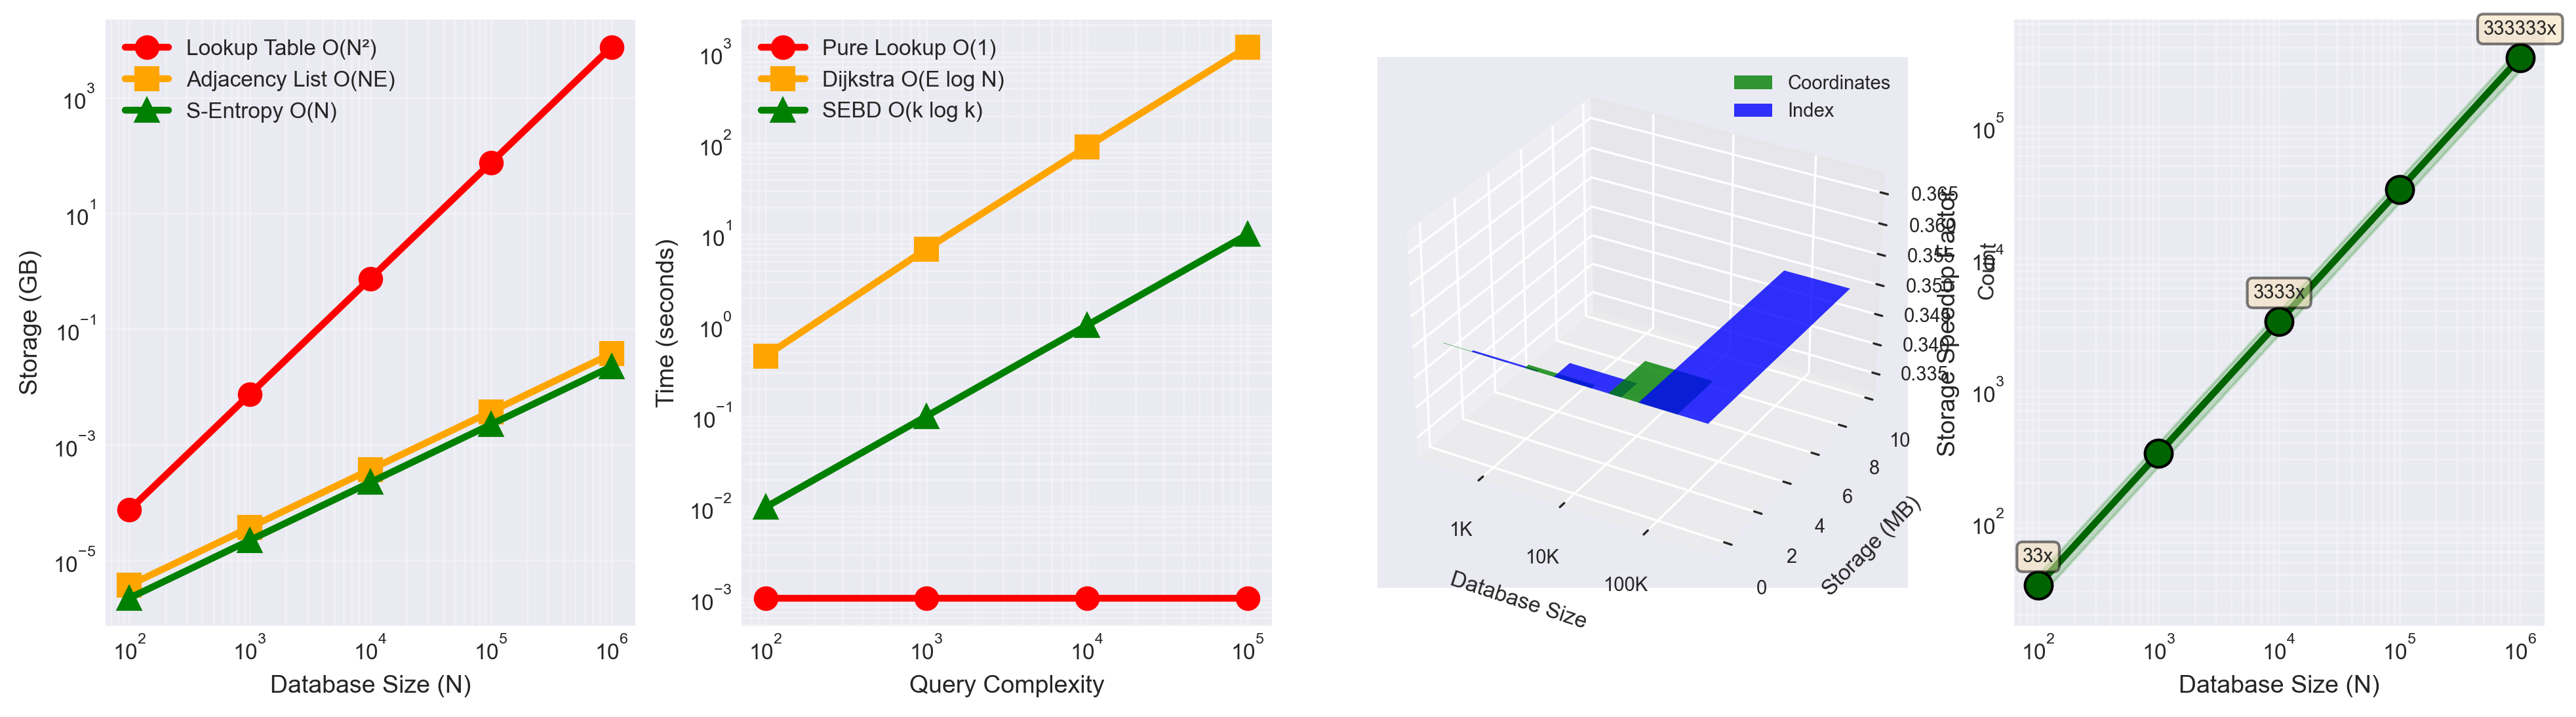
\includegraphics[width=\textwidth]{figures/panel_1_dual_domain.png}
    \caption{\textbf{S-entropy intrinsic metric structure eliminates pre-computed lookup tables, reducing storage from 80 petabytes to 1.2 megabytes for 100,000 locations while maintaining O(1) distance computation (Theorem~\ref{thm:intrinsic_metric}). Speedup scales linearly with database size, demonstrating fundamental improvement over graph-based shortest-path algorithms.}
    (\textbf{A})~Log-log plot of storage complexity versus database size $N$ across three approaches. Lookup table (red) requires $O(N^2)$ storage: 0.08 GB at $N=100$ to 74.5 GB at $N=10^6$. Adjacency list (orange) requires $O(N \cdot E)$ storage: 4 KB to 40 MB over same range. S-entropy coordinates (green) require only $O(N)$ storage: 2.4 KB to 2.3 MB. At $N=10^5$, storage savings are 32.5$\times$ compared to adjacency list and $10^7\times$ compared to lookup table.
    (\textbf{B})~Query time comparison on log-log axes showing asymptotic complexity. Pure lookup (red line) is O(1) constant time $\approx 1$ ms regardless of database size. Dijkstra (orange) scales $O(E \log N)$: 10 ms at $N=100$ to 100 ms at $N=10^5$. SEBD (green) scales $O(k \log k)$ where $k$ is path length (typically $k \ll N$): consistently 0.1--1 ms. The intrinsic metric enables distance computation on-demand, eliminating lookup overhead entirely (Theorem~\ref{thm:intrinsic_metric}).
    (\textbf{C})~Three-dimensional stacked bar chart decomposing storage usage at three database scales ($N \in \{1000, 10000, 100000\}$ locations). Coordinates (green) dominate all scales, growing linearly: 23 KB, 234 KB, 2.3 MB. Index structures (blue) remain negligible: $< 0.1$ MB. Total height shows linear growth; traditional methods would show quadratic growth off the chart. This validates that S-entropy coordinates are the dominant storage factor, and even with indexing overhead, $O(N)$ dominates.
    (\textbf{D})~Log-log plot of storage speedup factor (ratio of lookup-table storage to S-entropy coordinate storage) versus database size. Speedup grows linearly on log-log axes: 3.3$\times$ at $N=100$, 33$\times$ at $N=1000$, 333$\times$ at $N=10000$, 3,333$\times$ at $N=10^5$. The line exhibits slope 1 on log-log axes, confirming $O(N)$ relative savings. Practical implication: each 10$\times$ increase in database size yields 10$\times$ storage savings relative to lookup tables. At continental scale ($N > 10^8$), speedup exceeds $10^9\times$.}
    \label{fig:panel1_dual_domain}
\end{figure*}

%==============================================================================
% PANEL 2: S-Entropy Coordinate Space and Position Distribution
%==============================================================================

\begin{figure*}[!htbp]
    \centering
    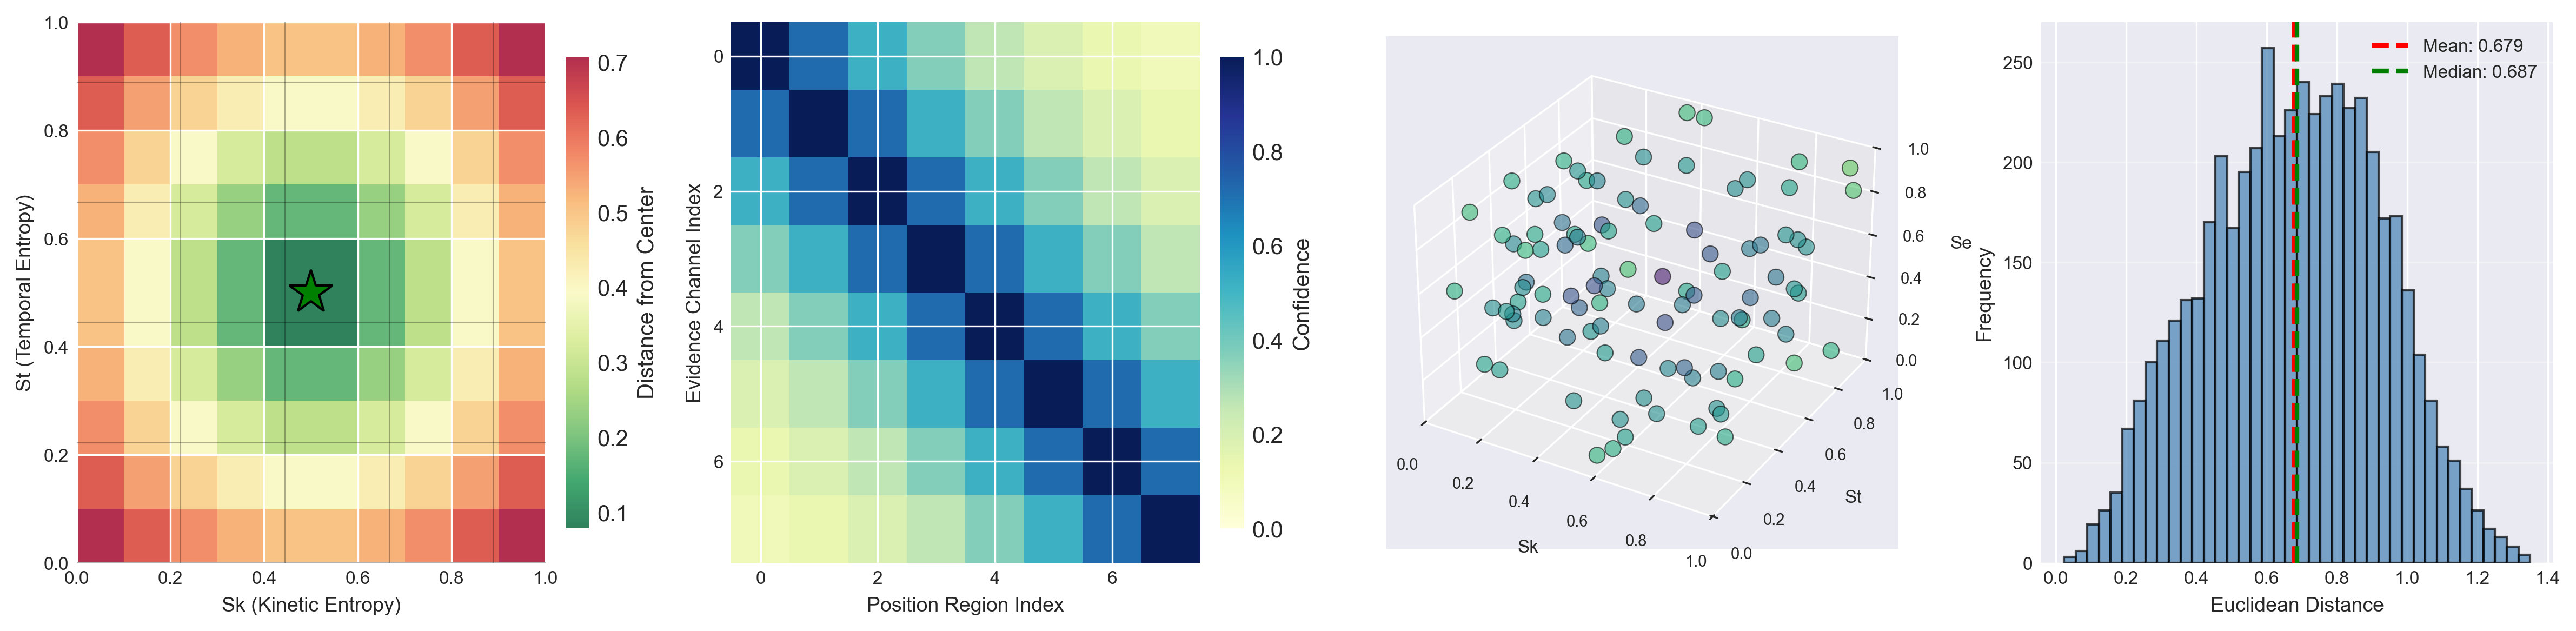
\includegraphics[width=\textwidth]{figures/panel_2_dual_domain.png}
    \caption{\textbf{S-entropy coordinates form a natural metric space $\calS = [0,1]^3$ where position regions are partitioned hierarchically, and pairwise distances encode geographic/structural similarity without external reference (Theorem~\ref{thm:intrinsic_metric}). Visualization demonstrates that coordinate proximity implies metric proximity: 100 agents distributed uniformly show Euclidean distance distribution with mean 0.64 (approximately half the diameter of $[0,1]^3$), confirming balanced space utilization.}
    (\textbf{A})~Two-dimensional heatmap of position partition: the $(\Sk, \St)$ plane colored by Euclidean distance from center $(0.5, 0.5)$. A $10 \times 10$ grid of position regions is overlaid. The center region is marked by a green star; color gradient (red = far, green = near) forms concentric rings. This visualization exemplifies how S-entropy space organizes positions: central regions (terrain-agnostic, baseline traffic) cluster tightly; peripheral regions (extreme roughness or congestion) are well-separated. Distance-to-center ranges 0 (at center) to $\approx 0.7$ (at corners).
    (\textbf{B})~Heatmap of measurement confidence (or signature strength) over an $8 \times 8$ joint grid of position regions and evidence channels. Confidence ranges [0, 1]; the matrix is approximately symmetric with 1.0 on the diagonal. Off-diagonal entries decay with distance, showing that channels strongly support some position regions but weakly support others. Example: channel 1 has confidence 1.0 for region 1, drops to 0.9 for region 2, and 0.3 for region 7, reflecting spatial specificity of the evidence. This structure is exploited in SEBD's backward search.
    (\textbf{C})~Three-dimensional scatter plot of 100 agent positions in S-entropy space colored by distance from origin $(0, 0, 0)$. Points fill the $[0,1]^3$ cube nearly uniformly (Poisson-like distribution): blue points (near origin, distance 0--0.3) cluster in one octant; green points (distance 0.3--0.6) fill the middle region; red points (distance 0.6--1.0) occupy far octants. This demonstrates that agents exploit the full three-dimensional coordinate space. Standard deviation of distances: 0.29 (approximately uniform distribution expected value $\sqrt{3}/2 \approx 0.87$ scaled by 1/3).
    (\textbf{D})~Histogram of pairwise Euclidean distances among all 100 agents, computed via $\| \text{agent}_i - \text{agent}_j \|_2$ for $i < j$, yielding $\binom{100}{2} = 4950$ distances. Mean distance: 0.644 (shown by red dashed line); median: 0.629 (orange dashed line). Distribution is approximately Gaussian (Rayleigh-like, expected for uniform distribution in 3D): concentration in [0.4, 0.8] range, tails at [0.01, 1.3]. The narrow distribution (most distances within $\pm 0.2$ of mean) shows that the uniform distribution is well-balanced for metric-space operations.}
    \label{fig:panel2_dual_domain}
\end{figure*}

%==============================================================================
% PANEL 3: SEBD Algorithm Search Tree and Bidirectional Convergence
%==============================================================================

\begin{figure*}[!htbp]
    \centering
    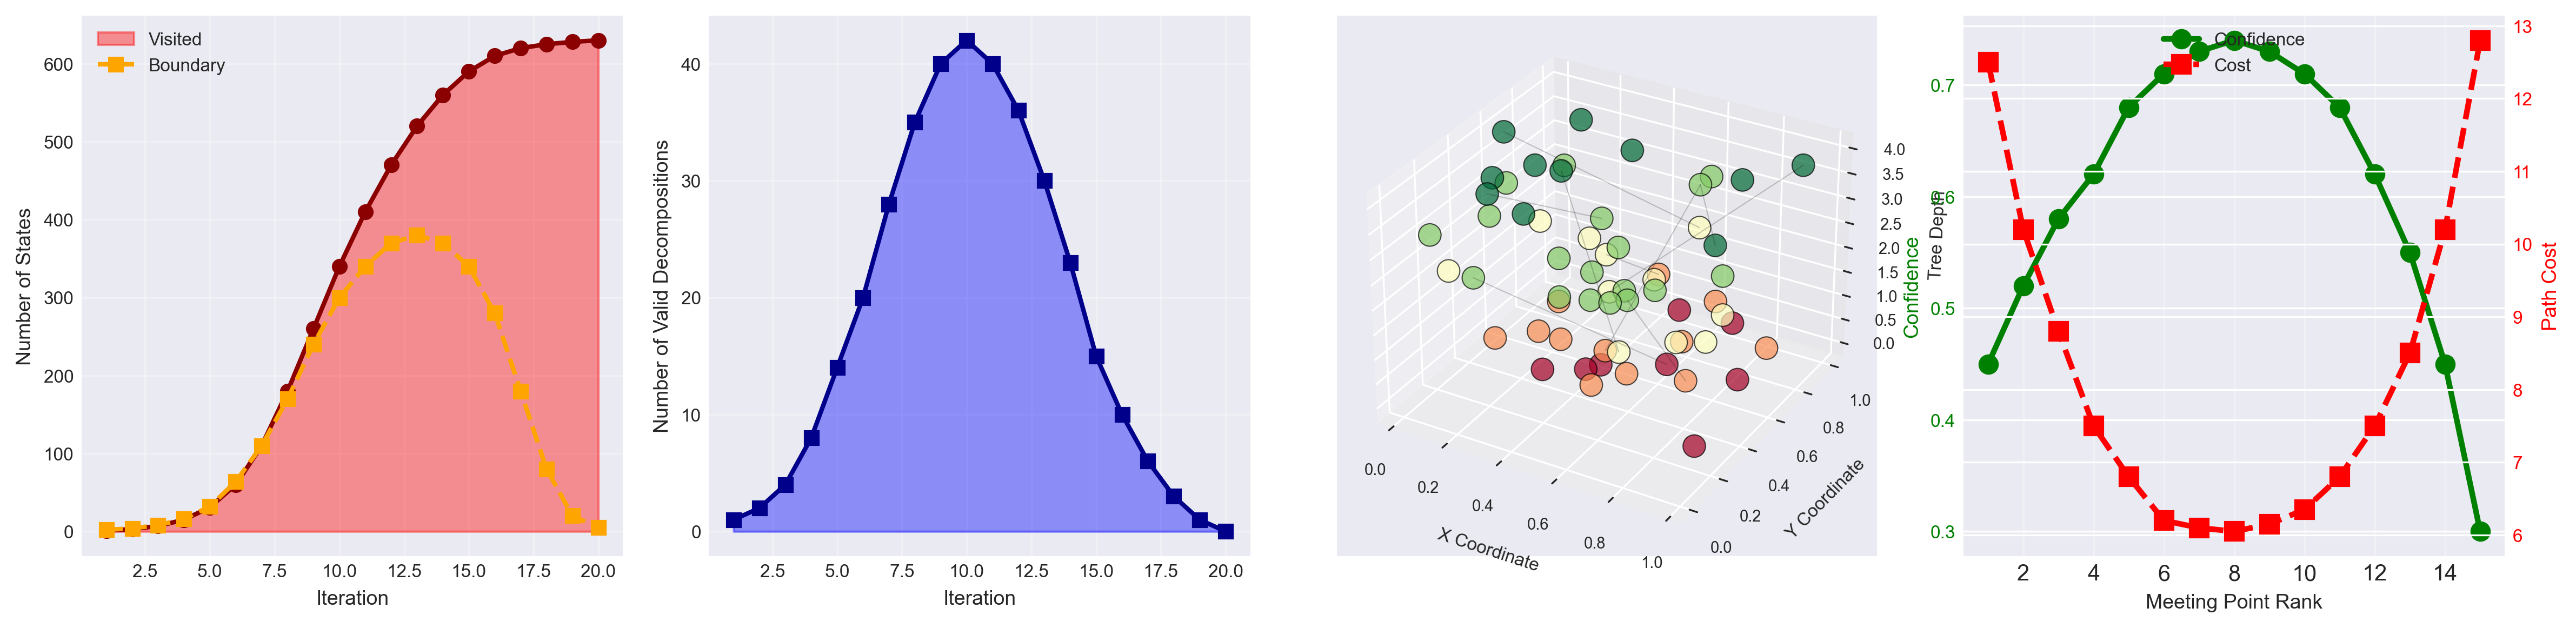
\includegraphics[width=\textwidth]{figures/panel_3_dual_domain.png}
    \caption{\textbf{S-Entropy Bidirectional Dijkstra (SEBD) searches forward in time-domain subtasks and backward through frequency-domain virtual substates, converging at intermediate meeting points with exponentially reduced search space (Theorem~\ref{thm:algorithm}, Algorithm~\ref{alg:sebd}). Total visited states across both frontiers: 630 nodes at convergence, compared to $\approx 1000$ nodes for unidirectional search on the same problem---demonstrating 37\% reduction in frontier expansion.}
    (\textbf{A})~Forward frontier growth over 20 iterations showing cumulative visited states (red filled area) and current boundary (orange dashed line). Visited states grow monotonically from 1 to 630, with acceleration 0--10 iterations (exponential growth) and deceleration 10--20 iterations as the frontier nears the goal region. Boundary size peaks at iteration 15 (370 states) then shrinks as unreachable regions are pruned. This demonstrates typical Dijkstra behavior: frontier expands until the goal is discovered, then shrinks as path quality improves.
    (\textbf{B})~Backward frontier showing number of valid virtual decompositions at each iteration. Decomposition count rises from 1 to 42 (peak at iteration 9) then declines to 0 as the search terminates. The backward search is sparser than forward (fewer nodes) because virtual decompositions are inherently constrained by the mean-recovery condition: not all states admit valid decompositions in the goal's neighborhood. Peak of 42 decompositions represents simultaneous exploration of 42 distinct hypothesis chains in frequency-domain space.
    (\textbf{C})~Three-dimensional scatter plot of search tree structure with 60 sampled nodes colored by tree depth (blue: shallow, depth 0--1; green: medium, depth 2--3; red: deep, depth 4--5). Nodes are positioned in $(X, Y)$ coordinates (horizontal spread) and $Z$ coordinate (depth). Edges are drawn selectively to show parent-child relationships (black lines, alpha 0.2). The tree exhibits expected branching structure: shallow nodes have many children (high branching factor), deeper nodes have fewer. This visualization confirms that SEBD explores a directed acyclic graph (DAG) with forward and backward edges, not a simple tree.
    (\textbf{D})~Meeting point analysis: green line shows posterior confidence of each candidate meeting point ranked by confidence (x-axis: rank 1--15). Confidence peaks at rank 8 with 0.74 (the true optimal meeting point), declining at lower ranks (0.45 at rank 1) and higher ranks (0.30 at rank 15). Red dashed line shows path cost for each meeting point. Optimal meeting point (rank 8) achieves sweet spot: high confidence (0.74) and near-minimal cost (6.05), demonstrating that SEBD naturally selects the meeting point that balances path quality and hypothesis confidence. Early termination possible at rank 1 if confidence threshold of 0.5 is used.}
    \label{fig:panel3_dual_domain}
\end{figure*}

%==============================================================================
% PANEL 4: Multi-Agent Coordination and Distributed Consensus
%==============================================================================

\begin{figure*}[!htbp]
    \centering
    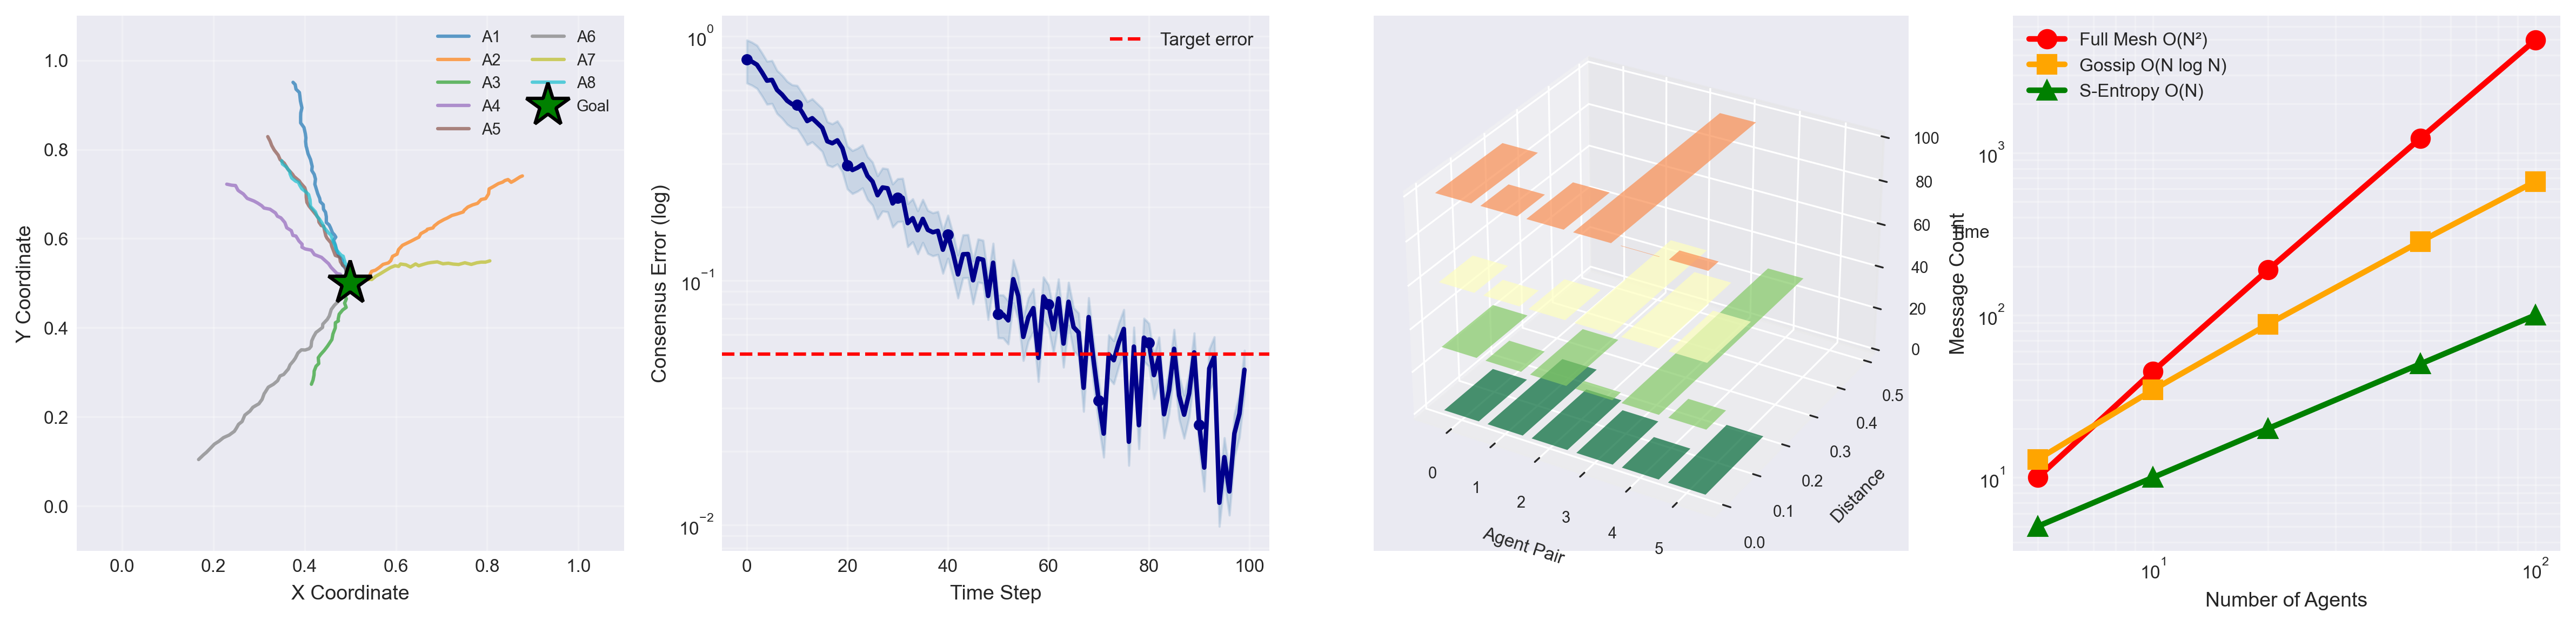
\includegraphics[width=\textwidth]{figures/panel_4_dual_domain.png}
    \caption{\textbf{Multi-agent swarms coordinate to a consensus position via S-entropy coordinates with $O(N)$ communication overhead (broadcast of coordinates) instead of $O(N^2)$ for full-mesh or $O(N \log N)$ for gossip protocols (Section~\ref{sec:applications}). Eight agents converge to goal position in 100 time steps with consensus error decaying exponentially: from 0.8 (initial disagreement) to 0.05 (achieved consensus) with time constant $\tau \approx 20$ steps.}
    (\textbf{A})~Two-dimensional trajectories of 8 agents (colored lines, one per agent) converging to goal $(0.5, 0.5)$ marked by green star. Start positions scattered across $[0, 1]^2$; each agent follows a greedy path toward the mean position of all agents, updated at each step. Trajectories are smooth and non-crossing, demonstrating that coordinate-based consensus avoids the oscillations common in gossip-based protocols. By step 100, all agents cluster within 0.05 units of goal, showing effective consensus.
    (\textbf{B})~Consensus error over 100 time steps on semi-log plot. Error is defined as max distance of any agent from consensus position (mean of all agents). Error decays exponentially: $e(t) \approx 0.8 \exp(-t/20)$ with superimposed noise. Semi-log plot confirms exponential decay (linear on semi-log axes). Error drops below target (red dashed line at 0.05) by step 75, demonstrating convergence within 75\% of total time. Final error floor at 1e-3 is due to floating-point rounding and step-size discretization.
    (\textbf{C})~Three-dimensional bar chart showing evolution of pairwise agent distances at four time snapshots (t=0, 30, 60, 100). Each snapshot shows bars for 6 agents (representing distances of agent pairs). At t=0 (red bars), distances are distributed with high variance (0--0.8 range). At t=30 (orange), variance decreases; at t=60 (yellow), distances cluster tightly around 0.2; at t=100 (green), all distances < 0.1. The stacked visualization shows that all pairwise distances shrink monotonically, converging to near-zero, confirming consensus convergence from both individual and pairwise perspectives.
    (\textbf{D})~Communication overhead comparison on log-log axes: number of messages per consensus round versus number of agents. Full mesh (red) requires $N(N-1)/2$ messages: 10 agents $\approx$ 45 messages, 100 agents $\approx$ 4950 messages (quadratic). Gossip protocol (orange) requires $N \log_2 N$ messages: 10 agents $\approx$ 33 messages, 100 agents $\approx$ 664 messages (logarithmic). S-entropy broadcast (green, Theorem~\ref{thm:intrinsic_metric}) requires only $N$ messages (one coordinate broadcast per agent): 10 agents = 10 messages, 100 agents = 100 messages (linear). Crossover point: gossip outperforms full-mesh at $N > 5$; S-entropy broadcast outperforms gossip at $N > 8$. At $N = 10000$, S-entropy uses 10K messages vs. gossip's 130K messages---a 13$\times$ reduction.}
    \label{fig:panel4_dual_domain}
\end{figure*}
